\section{Dataflow}

When designing a energy efficient system, dataflow is of great importance. The software 
on the MCU tries to minimize the number of data stores and movements. CPU usage is also
kept to a minimum as turning the CPU off conserves energy consumption.

\subsection{Peripherals}
The MCU facilitates audio I/O from ADC, DAC, SDCard and serial port interface to and from 
the FPGA. \todo{is serial audio I/O implemented}
\begin{figure}[h]
	\centering
	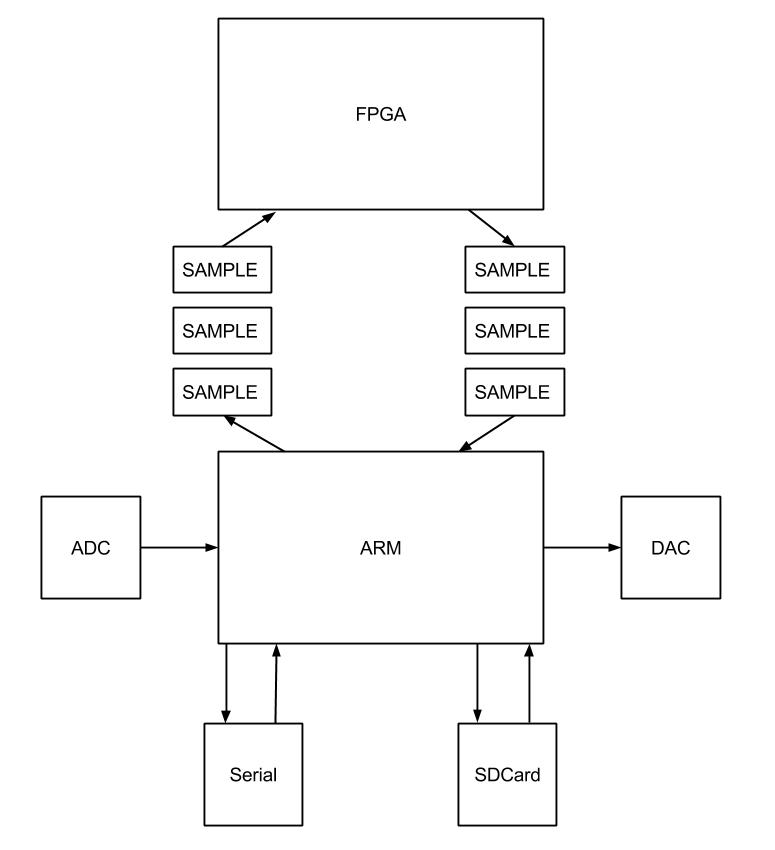
\includegraphics[height=150px]{figures/sw/sample-flow.png}
	%\begin{tikzpicture}[shorten >= 1pt, node distance=3cm, on grid, auto]
	%	\node[draw,rectangle,minimum size=2cm] (fpga) {FPGA};
	%	\node[draw,rectangle,below of=fpga,minimum size=2cm] (arm) {ARM};
	%\end{tikzpicture}
	\caption{Flow of samples}
	\label{fig:sw_sample_flow}
\end{figure}
\todo{Tikzify}


\subsection{External Bus Interface}
The MCU is connected to the FPGA and SRAM through the EBI. This leads to easy interfacing 
with these units as the EBI is memory mapped on the MCU. Communicating with the FPGA is 
done by reading and writing to memory. 

\todo{more about how the bus is implemented on the MCU}

\subsection{Direct Memory Access}
DMA provides the capability to move data without the intevention of the CPU. 
This is used extensively to implement the the dataflow in the low energy modes
that the MCU can run. The CPU is only used to configure and refresh the DMA 
channels inbetween tranfers. The MCU provides 12 independent DMA channels which can
move data between peripherals, RAM, Flash and the EBI. 

The core dataflow is from RAM on the MCU to the internal buffers on the FPGA 
and back to RAM on the MCU. For this four DMA channels are used.
\missingfigure{Figure showing RAM => FPGA => RAM}

In addition a DMA for each ADC and DAC are used when they are used as input and 
output respectively. When SDCard is used the contents of the files are read and
written by the CPU directly to and from RAM. 

\subsubsection{Deinterleaving of Samples}

Both when reading from a WAV file and from the ADC, samples from the
right and left channels are interleaved. The FPGA handles both channels in separat
pipelines. On the input side the samples has to be deinterleaved and on output they
are interleaved again. This is the reason for using two DMA channels for input and 
two for ouput. A complementary version of this procedure is implemented on the CPU 
and power comparison plots are included in the results section. \todo{Make sure they are} 
\missingfigure{Figure showing deinterleaving and interleaving}
The samples are deinterleaved by letting two DMA channels read from the same source d write to 
the pipelines for correct channel. The first DMA copies the samples for the left samples,
and start without a offset. The second DMA copies the samples for the right samples and 
start with an offset of one sample. Both DMAs read only every other sample and writes them
continuously to the FPGA input buffers. 

The interleaving process on output side works in the same way. The DMA reading from the
pipeline containing the left samples writes to the memory without a starting offset.
The right channel DMA writes with a offset by one sample. 

\subsubsection{Triggering Transfers}

All the DMA transfers are triggered by the use of one clock, the sample clock. This
clock is run at the sample speed (11kHz \todo{Lets update this to the correct one}), 
when using the DAC or ADC, or a arbritary frequency when doing SD to SD. The clock 
signal is fed into the Peripheral Reflex System of the MCU and propagates through the 
system using the following scheme 

\newpage
\begin{verbatim}
	
                        | Audio in
                        V
+------+  +-----+    +------+   +-----+     +--------+
|TIMER0|->| PRS |-+->| ADC0 |-->| DMA |---->| Buffer |
+------+  +-----+ |  +------+   +-----+     +--------+
                  |     .                      / \
                  |     .                     /   \
                  |     .                    V     V
                  |     .              +-----+     +-----+
                  |     +....irq......>| DMA |....>| DMA |
                  |                    +-----+     +-----+
                  |                       |           |
                  |                       V           V
                  |                   +------+    +-------+
                  |                   | FPGA |    | FPGA  |
                  |                   | Left |    | Right |
                  |                   +------+    +-------+
                  |                       |           |
                  |                       V           V
                  |                    +-----+     +-----+
                  |     +....irq......>| DMA |....>| DMA |
                  |     .              +-----+     +-----+
                  |     .                    \     /
                  |     .                     \   /
                  |     .                       V
                  |  +------+   +-----+     +--------+
                  +->| DAC0 |<--| DMA |<----| Buffer |
                     +------+   +-----+     +--------+
                        |
                        V Audio out
\end{verbatim} 

Here both the DAC and ADC consumes the PRS signal originated from TIMER0. The DMA copying 
from the ADC to the RAM buffer and the two DMAs performing the deinterleaving of the input
sampels receives a puls each time the ADC has buffered up $N$ samples. They then perform
a sequency of copy actions resulting in the input samples ending up inside the pipeline
buffers of the FPGA. On the other side the DAC sends a puls to the DMA that feeds it samples
in conjunction with the two DMAs performing the interleaving of the samples returned from the
FPGA pipelines.
